% The three recycling arms, side by side. PAPER_BRIEF §8.1: "the single most
% important explanatory diagram in the paper" -- a reader who follows this
% follows the whole experimental logic.
%
% What it has to make unmissable: k is not a design constant. It is read off the
% tau-dormant set at each event, in each layer, and then all three arms recycle
% exactly that many units. What differs across arms is only *which* k.
%
% Geometry note: TMLR's \textwidth is 6.5in = 16.5cm. Everything below is laid
% out to sit inside that -- 12 units at 0.5cm, arm labels to the left, wrapped
% notes to the right -- because a tikzpicture that overflows the margin is a
% silent error that only shows up in the PDF.
\begin{figure}[t]
\centering
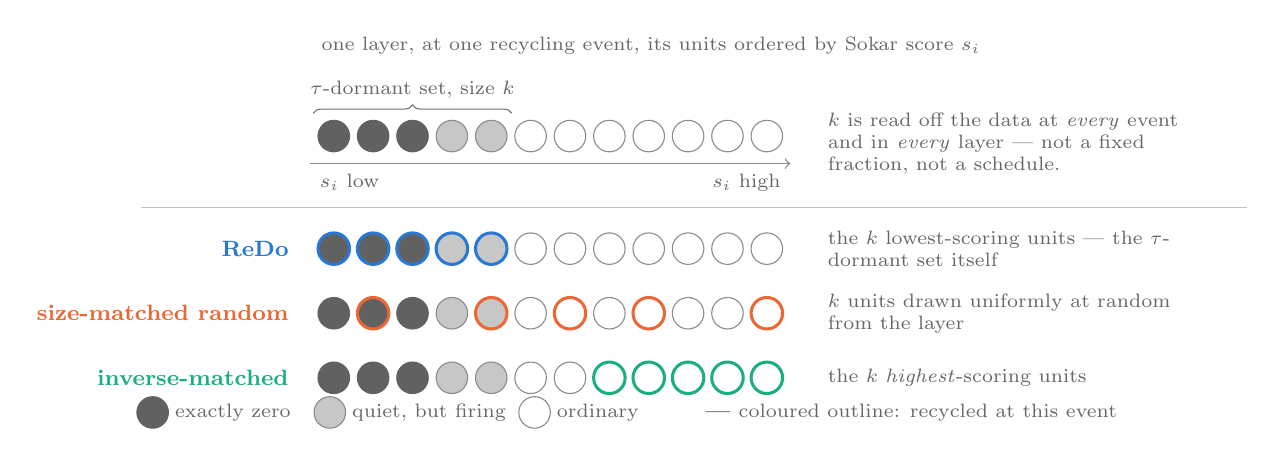
\begin{tikzpicture}[
  font=\small,
  unit/.style   = {circle, draw=black!45, minimum size=4.0mm, inner sep=0pt, line width=0.4pt},
  dead/.style   = {unit, fill=black!62, draw=black!62},
  quiet/.style  = {unit, fill=black!22, draw=black!45},
  alive/.style  = {unit, fill=white},
  pick/.style   = {draw=#1, line width=1.1pt},
  lbl/.style    = {font=\footnotesize\bfseries},
  sub/.style    = {font=\scriptsize, text=black!60},
  note/.style   = {font=\scriptsize, text=black!60, text width=45mm, align=left},
]

\definecolor{cRedo}{HTML}{2A78D6}
\definecolor{cRand}{HTML}{EB6834}
\definecolor{cInv}{HTML}{1BAF7A}

\def\ux{0.50}          % unit pitch
\def\xend{5.50}        % 11 * \ux
\def\xnote{6.15}       % where the right-hand notes start

% ---- the score ordering, shared by all three panels ---------------------------
\node[sub, anchor=west] at (-0.28,2.30)
  {one layer, at one recycling event, its units ordered by Sokar score $s_i$};

\draw[decorate, decoration={brace, amplitude=3pt}, black!55]
  (-0.26,1.44) -- (4*\ux+0.26,1.44)
  node[midway, above, sub, yshift=0.6mm] {$\tau$-dormant set, size $k$};

\foreach \i in {0,...,11}{
  \pgfmathsetmacro\xx{\i*\ux}
  \ifnum\i<3 \node[dead]  at (\xx,1.15) {}; \else
  \ifnum\i<5 \node[quiet] at (\xx,1.15) {}; \else
             \node[alive] at (\xx,1.15) {}; \fi\fi
}
\draw[->, black!45, line width=0.5pt] (-0.30,0.80) -- (\xend+0.30,0.80);
\node[sub, anchor=west] at (-0.30,0.56) {$s_i$ low};
\node[sub, anchor=east] at (\xend+0.30,0.56) {$s_i$ high};

\node[note, anchor=west] at (\xnote,1.05)
  {$k$ is read off the data at \emph{every} event and in \emph{every} layer ---
   not a fixed fraction, not a schedule.};

\draw[black!25, line width=0.4pt] (-2.45,0.24) -- (11.6,0.24);

% ---- the three arms ----------------------------------------------------------
\def\rowy{-0.28}
\foreach \arm/\name/\col/\sel/\note in {%
  0/ReDo/cRedo/{0,1,2,3,4}/{the $k$ lowest-scoring units --- the $\tau$-dormant set itself},
  1/size-matched random/cRand/{1,4,6,8,11}/{$k$ units drawn uniformly at random from the layer},
  2/inverse-matched/cInv/{7,8,9,10,11}/{the $k$ \emph{highest}-scoring units}%
}{
  \pgfmathsetmacro\yy{\rowy - \arm*0.82}
  \node[lbl, anchor=east, text=\col] at (-0.45,\yy) {\name};
  \foreach \i in {0,...,11}{
    \pgfmathsetmacro\xx{\i*\ux}
    \ifnum\i<3 \node[dead]  at (\xx,\yy) {}; \else
    \ifnum\i<5 \node[quiet] at (\xx,\yy) {}; \else
               \node[alive] at (\xx,\yy) {}; \fi\fi
  }
  \foreach \s in \sel {\node[unit, pick=\col] at (\s*\ux,\yy) {};}
  \node[note, anchor=west] at (\xnote,\yy) {\note};
}

% ---- legend ------------------------------------------------------------------
\def\ly{-2.36}
\node[dead]  at (-2.30,\ly) {}; \node[sub, anchor=west] at (-2.14,\ly) {exactly zero};
\node[quiet] at (-0.05,\ly) {}; \node[sub, anchor=west] at ( 0.11,\ly) {quiet, but firing};
\node[alive] at ( 2.55,\ly) {}; \node[sub, anchor=west] at ( 2.71,\ly) {ordinary};
\node[sub, anchor=west] at (4.55,\ly)
  {\,\textbf{---} coloured outline: recycled at this event};

\end{tikzpicture}
\caption{\textbf{The three recycling arms.} At every event, in every layer, the
$\tau$-dormancy score is computed and $k$ is set to the size of the
$\tau$-dormant set. All three arms then recycle exactly $k$ units by the
identical procedure --- re-initialise the incoming weights from the layer's
original initialisation distribution, zero the outgoing weights
\citep{sokar2023dormant} --- and differ only in \emph{which} $k$. Because $k$ is
recomputed per layer per event rather than fixed as a fraction or a schedule,
the comparison isolates the effect of targeting from the effect of dose. Circles
are units; their shading is the state measured on the probe batch, which is
independent of the score that selects them.}
\label{fig:arms}
\end{figure}
